\documentclass{article}

\usepackage[utf8]{inputenc}

\usepackage{graphicx}
\usepackage{tikz}
\usepackage{pgfplots}
\usepackage{pgf-pie}

\usetikzlibrary{arrows.meta}
\pgfplotsset{compat=1.18}

\begin{document}

%=========================
% Gráfico 1: Exposición a desinformación por canal
%=========================
\section*{Gr\'afico 1: Exposici\'on a desinformaci\'on por canal}

\begin{center}
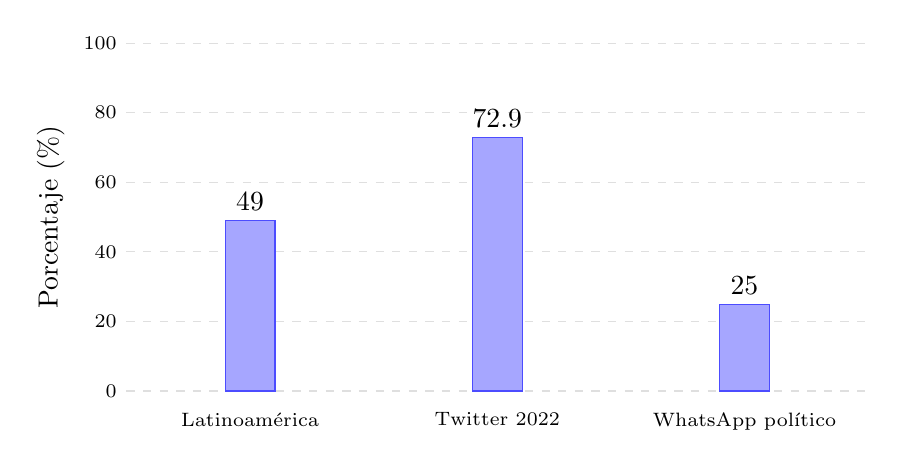
\begin{tikzpicture}
\begin{axis}[
    ybar,
    bar width=18pt,
    ymin=0, ymax=100,
    ylabel={Porcentaje (\%)},
    symbolic x coords={Latinoam\'erica,Twitter 2022,WhatsApp pol\'itico},
    xtick=data,
    tick label style={font=\scriptsize},
    enlarge x limits=0.25,
    nodes near coords,
    nodes near coords align={vertical},
    width=11cm,
    height=6cm,
    ymajorgrids,
    grid style={dashed,gray!25},
    axis line style={draw=none},
    ytick style={draw=none},
    xtick style={draw=none}
]
\addplot[
    fill=blue!35,
    draw=blue!70
] coordinates {
    (Latinoam\'erica,49)   % ven noticias falsas a diario
    (Twitter 2022,72.9)    % vieron info falsa sobre plebiscito
    (WhatsApp pol\'itico,25) % mensajes con desinfo
};
\end{axis}
\end{tikzpicture}
\end{center}

%=========================
% Gráfico 2: Percepción del riesgo y apoyo a regulación
%=========================
\section*{Gr\'afico 2: Percepci\'on del riesgo y apoyo a regular}

\begin{center}
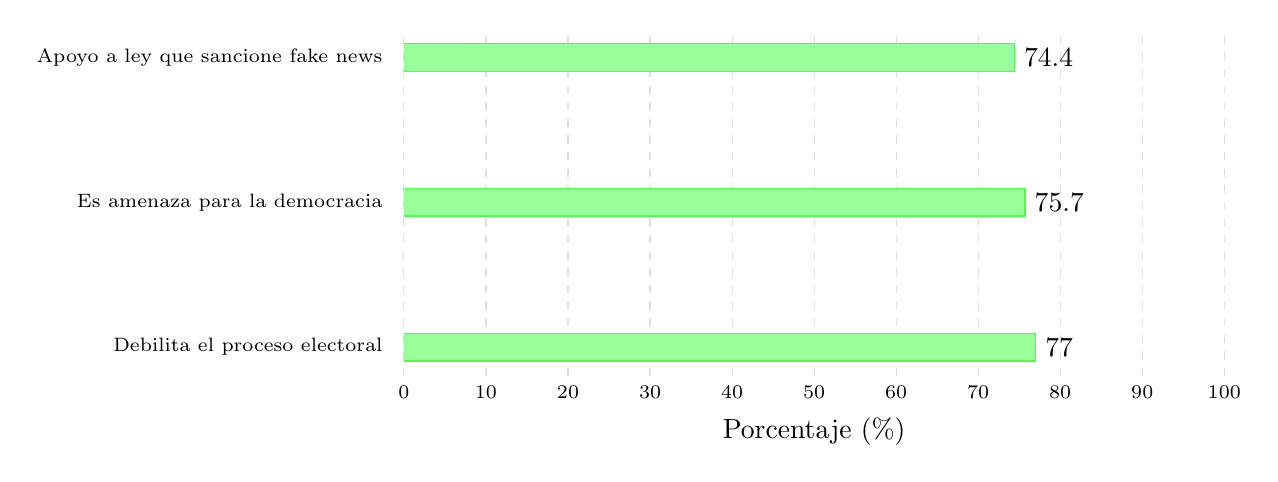
\begin{tikzpicture}
\begin{axis}[
    xbar,
    xmin=0, xmax=100,
    xlabel={Porcentaje (\%)},
    symbolic y coords={
        Debilita el proceso electoral,
        Es amenaza para la democracia,
        Apoyo a ley que sancione fake news},
    ytick=data,
    tick label style={font=\scriptsize},
    width=12cm,
    height=6cm,
    nodes near coords,
    nodes near coords align={horizontal},
    xmajorgrids,
    grid style={dashed,gray!25},
    axis line style={draw=none},
    xtick style={draw=none},
    ytick style={draw=none}
]
\addplot[
    fill=green!40,
    draw=green!70
] coordinates {
    (77,Debilita el proceso electoral)
    (75.7,Es amenaza para la democracia)
    (74.4,Apoyo a ley que sancione fake news)
};
\end{axis}
\end{tikzpicture}
\end{center}

%=========================
% Gráfico 3: Línea de tiempo 2016–2025
%=========================
\section*{Gr\'afico 3: L\'inea de tiempo 2016--2025}

\begin{center}
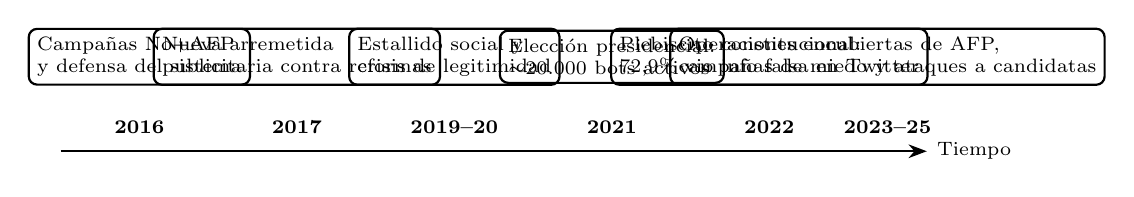
\begin{tikzpicture}[
    >=Stealth,
    event/.style={rectangle, rounded corners=3pt, draw, thick,
                  align=left, font=\scriptsize, inner sep=3pt},
    year/.style={font=\scriptsize\bfseries}
]

% L\'inea base
\draw[->, thick] (0,0) -- (11,0) node[right, font=\scriptsize] {Tiempo};

% 2016
\node[year]  at (1,0.3)  {2016};
\node[event] at (1,1.2)  {Campa\~nas No+AFP\\y defensa del sistema};

% 2017
\node[year]  at (3,0.3)  {2017};
\node[event] at (3,1.2)  {Nueva arremetida\\publicitaria contra reformas};

% 2019--2020
\node[year]  at (5,0.3)  {2019--20};
\node[event] at (5,1.2)  {Estallido social y\\crisis de legitimidad};

% 2021
\node[year]  at (7,0.3)  {2021};
\node[event] at (7,1.2)  {Elecci\'on presidencial:\\$\sim$20.000 bots activos};

% 2022
\node[year]  at (9,0.3)  {2022};
\node[event] at (9,1.2)  {Plebiscito constitucional:\\72{,}9\% vio info falsa en Twitter};

% 2023--25
\node[year]  at (10.5,0.3) {2023--25};
\node[event] at (10.5,1.2) {Operaciones encubiertas de AFP,\\
campa\~nas de miedo y ataques a candidatas};

\end{tikzpicture}
\end{center}

%=========================
% Gráfico 4: Ataques según género (pie / donut)
%=========================
\section*{Gr\'afico 4: Ataques seg\'un g\'enero}

\begin{center}
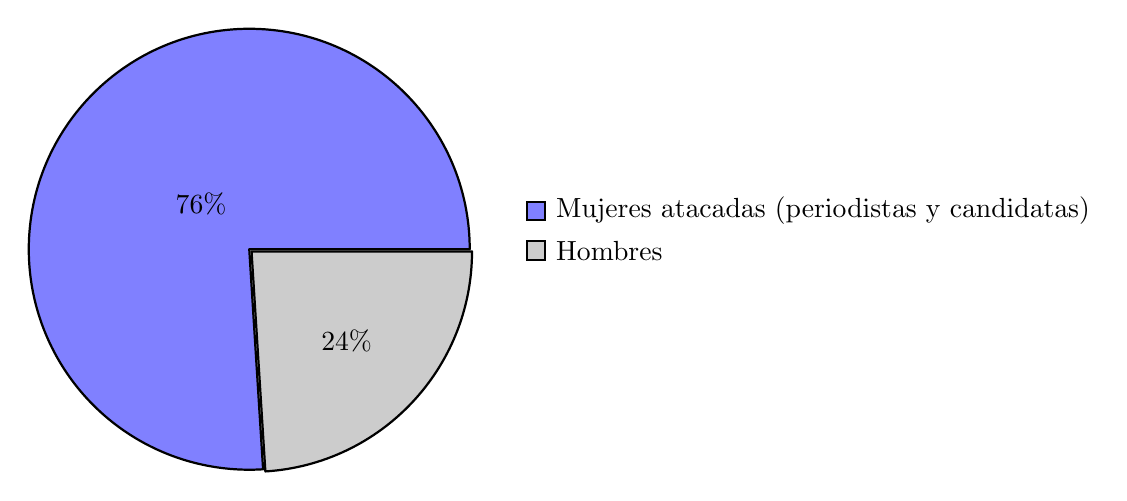
\begin{tikzpicture}
\pie[
    radius=2.8,
    text=legend,
    color={blue!50, gray!40},
    explode=0.02
]{
    76/Mujeres atacadas (periodistas y candidatas),
    24/Hombres
}
\end{tikzpicture}
\end{center}

\newpage

%=========================
% Gráfico 5: Polarización subjetiva (percepción vs realidad)
%=========================
\section*{Gr\'afico 5: Polarizaci\'on subjetiva sobre aborto en la derecha}

\begin{center}
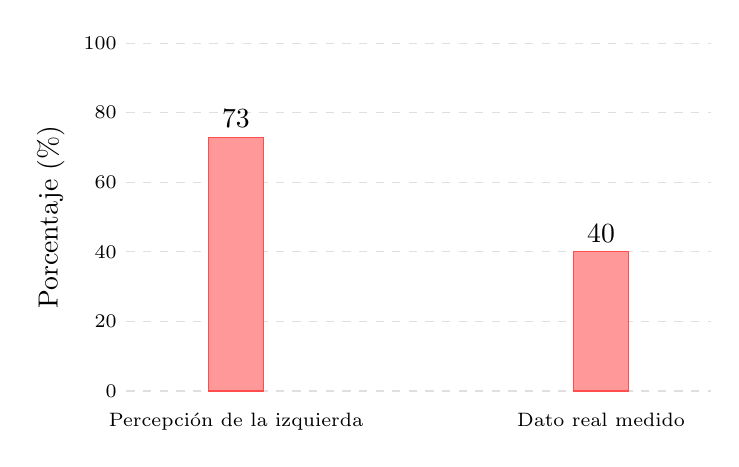
\begin{tikzpicture}
\begin{axis}[
    ybar,
    bar width=20pt,
    ymin=0, ymax=100,
    ylabel={Porcentaje (\%)},
    symbolic x coords={Percepci\'on de la izquierda,Dato real medido},
    xtick=data,
    tick label style={font=\scriptsize},
    enlarge x limits=0.3,
    nodes near coords,
    nodes near coords align={vertical},
    width=9cm,
    height=6cm,
    ymajorgrids,
    grid style={dashed,gray!25},
    axis line style={draw=none},
    ytick style={draw=none},
    xtick style={draw=none}
]
\addplot[
    fill=red!40,
    draw=red!70
] coordinates {
    (Percepci\'on de la izquierda,73)
    (Dato real medido,40)
};
\end{axis}
\end{tikzpicture}
\end{center}

%=========================
% Gráfico 6: Flujo de influencia AFP → campañas → bots → ciudadanía
%=========================
\section*{Gr\'afico 6: Flujo de influencia de la desinformaci\'on}

\begin{center}
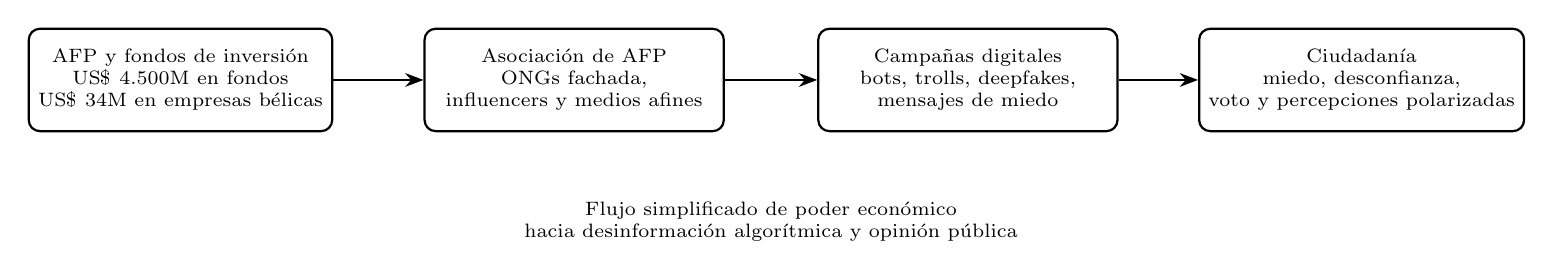
\begin{tikzpicture}[
    box/.style={rectangle, rounded corners=4pt, draw, thick,
                align=center, font=\scriptsize, minimum width=3.8cm,
                minimum height=1.3cm},
    >=Stealth
]

% Nodos en l\'inea
\node[box] (afp) at (0,0)
    {AFP y fondos de inversi\'on\\US\$ 4.500M en fondos\\US\$ 34M en empresas b\'elicas};

\node[box] (asoc) at (5,0)
    {Asociaci\'on de AFP\\ONGs fachada,\\influencers y medios afines};

\node[box] (bots) at (10,0)
    {Campa\~nas digitales\\bots, trolls, deepfakes,\\mensajes de miedo};

\node[box] (cit)  at (15,0)
    {Ciudadan\'ia\\miedo, desconfianza,\\voto y percepciones polarizadas};

% Flechas
\draw[->, thick] (afp) -- (asoc);
\draw[->, thick] (asoc) -- (bots);
\draw[->, thick] (bots) -- (cit);

% Texto explicativo
\node[font=\scriptsize, align=center] at (7.5,-1.8)
    {Flujo simplificado de poder econ\'omico\\
     hacia desinformaci\'on algor\'itmica y opini\'on p\'ublica};

\end{tikzpicture}
\end{center}

\end{document}
